
\taskpic{ Прямоугольная рамка расположена в плоскости бесконечного
  прямолинейного проводника с током, причём стержни $AD$ и $BC$
  параллельны проводнику. В середину стороны $BC$ включен прибор,
  измеряющий протекший заряд. Рамку можно перевести в новое положение,
  отмеченное на рисунке пунктиром, двумя способами: 1) перемещая её
  параллельно самой себе; 2) вращая вокруг $BC$ на $180^{\circ}$. В
  каком случае заряд, протекший через прибор, больше? }
{
  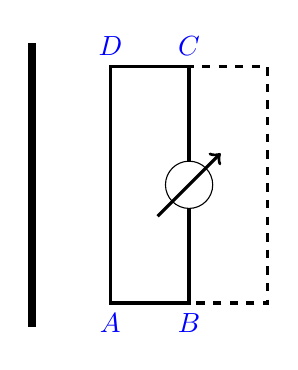
\begin{tikzpicture}
    \draw[line width=0.1cm] (0,-0.3) -- (0,3.3);
    \draw[very thick] (1,0) node[below,blue] {$A$} -- (1,3)
    node[above,blue] {$D$} -- (2,3) node[above,blue] {$C$} -- (2,0)
    node[below,blue] {$B$} -- cycle;
    \draw[very thick,dashed] (2,0) -- (2,3) -- (3,3) -- (3,0) --
    cycle;
    \draw[fill=white] (2,1.5) circle (0.3cm);
    \draw[very thick,->] (1.6,1.1) -- (2.4,1.9);
  \end{tikzpicture}
}
% Слободецкий, Асламазов (Капица), №183